\chapter{Materials and Methods}
\label{sec:MaterialsAndMethods}
This document contains two appendices: A and B. Figures and Tables in Appendix A begin with the prefix `A', and Section numbers with `5'. 
The Figures and Tables in Appendix B begin with the prefix `B', and Section numbers with `6'. 

\section{Sourcing of samples}

\noindent Tables \ref{appendix:sequenceInfo} and \ref{appendix:issr_sample_table} contain detailed lists of all the samples used in this study. Outgroup and additional ingroup sequences were obtained from Genbank to supplement the dataset, and are listed in Table \ref{appendix:outgroups}.

\subsection{South Africa}

\subsubsection{Wild populations} 
\textit{Dactylopius opuntiae} samples were collected from wild populations on \textit{Opuntia ficus-indica} and \textit{Opuntia engelmannii} from various locations in the Eastern Cape Province. These are known to be the `ficus' lineage. 

\subsubsection{Uitenhage Mass Rearing Facility} 
 The Uitenhage Mass Rearing Facility in the Eastern Cape Province rears six insect agents for the control of invasive Cactaceae in the country. Four of these are \textit{Dactylopius} species, and were included in the analyses of this project. These were \textit{D. austrinus}, \textit{D. tomentosus} `imbricata', \textit{D. ceylonicus}, and \textit{D. opuntiae} `stricta' (more information is available at the Centre for Biological Control (CBC) Website, at \url{https://www.ru.ac.za/centreforbiologicalcontrol/massrearing/uitenhagemassrearingfacility/}). \\
As there are wild populations of the `ficus' \textit{D. opuntiae} lineage on \textit{O. ficus-indica} cacti in the surrounding vicinity, it is a concern as to whether this lineage is hybridising with the desired `stricta' lineage reared inside the facility. It is known that these two lineages can hybridise, which affects the host-specificity of offspring.
`Stricta' samples were collected from the facility and compared to original `stricta' source population samples and to `ficus' specimens to determine whether hybridisation had occurred. Individuals of the `stricta' lineage from the original stock imported from Australia were kept by Hildegard Klein and John Hoffmann (biological control specialists), and were used as a benchmark for the identification of this lineage.

\subsubsection{\textit{Dactylopius tomentosus} `cholla'} 
The \textit{Dactylopius tomentosus} `cholla' lineage was sourced from \textit{Cylindropunita fulgida} var. \textit{mammilata} in the Kirstenbosch Cape Town Botanical Gardens. Additional samples collected from \textit{C. fulgida} var. \textit{mammilata} in Jansenville in the Eastern Cape Province required identification confirmation, and were included in the analyses. 

\subsubsection{Kruger National Park}
\textit{Opuntia stricta} is the most widespread IAP in the Kruger National Park (KNP), covering approximately 35 000 ha surrounding Skukuza \citep{lotter1998integrated, foxcroft2004reconstructing}. It was first recorded in the Skukuza staff village in 1953, and spread rapidly within the subsequent decades \citep{lotter1998integrated}.
% Mechanical control attempts began in 1985 with the use of herbicides \citep{foxcroft2003Kruger}, but this was unsuccessful due to the survival of soil-stored seeds and small plants that had been overlooked, and the lack of follow-up work \citep{hoffmann1998long, foxcroft2004reconstructing}. 
% Biological control initiatives began in 1988 with the release of the phycitid moth \textit{Cactoblastis cactorum}, which provided a moderate level of control by stinting plant growth and reducing the time taken for plants to reach sexual maturity \citep{Hoffmann1998EvaluationAfrica, hoffmann1998long}.
\textit{Dactylopius opuntiae} was released on three separate occasions between 1990 and 1995, but did not establish on the weed \citep{lotter1998integrated, foxcroft2000dispersal}. This was because it was the `ficus' lineage, which does not establish on \textit{O. stricta} \citep{Volchansky1999}. The `stricta' lineage was subsequently imported from an Australian stock and released in the KNP in 1997, and has provided a substantial level of control \citep{lotter1998integrated, foxcroft2000dispersal}.
\textit{Dactylopius opuntiae} samples were obtained from Skukuza in the KNP in 2018 in order to confirm whether they were still of the original `stricta' lineage released in 1997. 

\subsection{Namibia}
\textit{Dactylopius opuntiae} samples were collected from \textit{O. ficus-indica} and \textit{O. stricta}. These were expected to be the `ficus' lineage, as this was the only lineage intentionally released in the country in 1975 and 1980 \citep{brown1985invasive, paterson2019prospects}. The first release in 1975 was for the control of \textit{O. stricta}, but the `ficus' lineage did not establish \citep{brown1985invasive} due to it being the incorrect agent. This is another example of the importance of correct identification. Additionally, two samples collected on an unidentified \textit{Harrisia} sp. in Windhoek were included in the present analysis. It was unexpected to find \textit{D. opuntiae} `ficus' on a \textit{Harrisia} cactus, and so further identification was required. 
\subsection{The USA}
\textit{Dactylopius} populations were collected from ten different \textit{O. engelmannii} lineages across the southern states of Arizona, New Mexico, Texas, and California in 2017 \citep{isbcw2018byrne}, and were identified morphologically as \textit{D. opuntiae}. These are currently in quarantine at the University of the Witwatersrand in Johannesburg, and are being tested for their use as additional biological control agents for \textit{O. engelmannii}. Samples from each lineage were included in the present genetic analysis.
Additional confirmed \textit{D. confusus} specimens were sourced from the Entomology Department at the University of Arizona, and included in the analysis for comparison. This is because \textit{D. opuntiae} and \textit{D. confusus} are frequently confused, as they are often found on the same individual host plant. Genetic analyses could therefore confirm the morphological identifications made for these ten lineages.

\subsection{Australia}
There are eight naturalised \textit{Cylindropuntia} species in Australia; namely \textit{C. fulgida} var. \textit{mamillata} ((D. C.) Backeberg), \textit{C. imbricata} (Haworth) F. M. Knuth, \textit{C. kleiniae} (D. C.) F. M. Knuth, \textit{C. leptocaulis} (D. C.) F. M. Knuth, \textit{C. prolifera} (Engelm.) F. M. Knuth, \textit{C. rosea} (D. C.) Backeberg, \textit{C. spinosior} (Engelm.) F. M. Knuth, and \textit{C. tunicata} (Lehm.) F. M. Knuth \citep{Jones2015}. All of these species negatively impact the environment, agricultural practices, and recreational activities \citep{Lloyd2014, Jones2015}. The Australians have imported 20 \textit{D. tomentosus} lineages into the country to serve as potential biocontrol agents \citep{isbcw2018Jones}, of which the `bigelovii', `acanthocarapa x echinocarpa', `cylindropuntia sp.', `imbricata', `cholla', and `californica' lineages
were obtained from Michael Day at the Department of Agriculture, Fisheries and Forestry, (Biosecurity Queensland) for inclusion in this project. These lineages are the most damaging to target weeds, and are in the process of, or have already been, released. Additional \textit{D. austrinus}, \textit{D. ceylonicus}, and \textit{D. opuntiae} specimens were included as well, which are commonly used biological control agents in Australia for Cactaceae, and have been established in the country for many years.

\subsection{Saudi Arabia}

\textit{Dactylopius opuntiae} samples collected from \textit{Opuntia stricta} were sourced from four localities in the Jazan Region of Saudi Arabia; namely Aldyer, Jazan City, Hurob, and Alaredah. Confirmation was required that these belonged to the `stricta' lineage, because this particular lineage provides the greatest level of control for \textit{O. stricta} weeds.

% Scanning electron microscope (SEM) images were taken of \textit{Dactylopius austrinus}, \textit{D. ceylonicus}, \textit{D. tomentosus} `imbricata' and `cholla' and \textit{D. opuntiae} `ficus' (images are in the \hyperref[appendix:semImages]{Appendix}). 

\section{Sample preservation and DNA extraction}
All specimens were preserved in 95\% ethanol and stored at -18\textsuperscript{o}C. Microscope slides of selected specimens were prepared according to the methods of \citet{Ben-Dov1997}. 
Buffer ATL (tissue lysis buffer) (Qiagen\textsuperscript{\textcopyright}) and Proteinase K (Qiagen\textsuperscript{\textcopyright}) were used to digest insect tissue, followed by a standard salt extraction procedure \citep{Bruford1992} (See Section \ref{appendix:extractionProtocol} for the detailed protocol). DNA pellets were resuspended in 100 $\mu$L AE (elution) buffer (Qiagen\textsuperscript{\textcopyright}) and stored at -18\textsuperscript{o}C. The concentration and purity of DNA extracts were ascertained through the use of a ThermoScientific Nanodrop 2000 spectrophotometer. When present, carminic acid residues in the extracts affected spectrometry and DNA concentration readings, but did not inhibit the successful amplification of target fragments.  

\section{DNA sequencing}

\subsection{Gene regions}

Three gene regions were amplified; namely the mitochondrial cytochrome oxidase subunit 1 (COI) region and 12S ribosomal (12S rRNA) region, and the nuclear 18S ribosomal (18S rRNA) region. 
% Mitochondrial DNA (mtDNA) is a double-stranded circular molecule ranging between 15 and 18 kb in length; containing 37 genes as well as non-coding regions \citep{Cameron2014InsectPhylogeny}. It makes up about 1 to 2\% of the total DNA in a cell \citep{Yang2014}. The coding gene region comprises of 13 protein coding, 22 transfer RNA (tRNA) and 2 ribosomal RNA (rRNA) genes \citep{Yang2014,Cameron2014InsectPhylogeny}. 
Mitochondrial DNA is maternally inherited, and is highly conserved across the insect orders and bilaterian animals as a whole \citep{Hoy2013, Cameron2014InsectPhylogeny}. This high level of conservation makes it particularly useful for phylogenetic studies \citep{Lunt1996, Hoy2013, DeMandal2014}. Another useful property of mtDNA is that different gene regions mutate at different rates, allowing for greater analytical potential \citep{Hoy2013}. 
% The COI mitochondrial gene encodes for the production of subunit 1 of the cytochrome c oxidase enzyme \citep{Lunt1996}. This enzyme plays an important role in cellular respiration by acting as both an electron transporter and translocator of protons across the cell membrane \citep{Lunt1996}. \citet{Yang2014} showed how conserved this gene is across organisms as disparate as humans and bacteria. 
The third position nucleotides of the COI gene display a high rate of base substitutions (`wobble'), leading to a mutation rate about three times faster than that of the 12S and 16S rDNA genes \citep{Knowlton1998}. This rapid rate of gene evolution has been found to be useful in using genetic barcoding to discriminate between phylogeographic lineages within the same species \citep{Cox2001, Gentekaki2012}. \\
% The 12S mitochondrial gene encodes for the production of rRNA, which translates mRNA into mitochondrial proteins \citep{Yang2014}. The 18S nuclear gene also encodes for the production of rRNA, which makes up the small ribosomal subunit \citep{Meyer2010}. 
The 18S gene is one of the slowest-evolving nuclear sequences, and is useful for assessing the ancestral relationships between organisms \citep{Hillis1991}. \citet{Campana2015} did not find any variation between the 18S markers across \textit{D. coccus} lineages, and hence discarded them from their study. The present study however used this gene because it involved a multi-species analysis.

\subsection{Polymerase Chain Reaction (PCR)}

Forward and reverse primers were used according to the methods of
\citet{Park2010RecoveryPrimers}, \citet{Campana2015}, and \citet{Mathenge2015} (Table \ref{tab:primers}). 

\vspace{0.5cm}

\begin{table}[H]
\renewcommand{\arraystretch}{0.6}
\centering
\caption{Primers used for the amplification of the COI, 12S, and 18S gene regions in \textit{Dactylopius} species.} 
\label{tab:primers} 
\begin{tabular}{@{}lll@{}}
\toprule
\multicolumn{1}{c}{\textbf{Gene}} & \multicolumn{1}{c}{\textbf{Primer pair (5' $\rightarrow$ 3')}} & \multicolumn{1}{c}{\textbf{Reference}} \\ \midrule
\multirow{4}{*}{\textbf{COI-A}} & \textbf{Forward (PcoF1)} & \citet{Park2010RecoveryPrimers} \\
 & CCTTCAACTAATCATAAAAATATYAG &  \\
 & \textbf{Reverse (LepR1)} &  \\
 & TAAACTTCTGGATGTCCAAAAAATCA &  \\ \hline
\multirow{4}{*}{\textbf{COI-B}} & \textbf{Forward (DTOMf )} & \citet{Mathenge2015} \\
 & TCCGRATAGAACTWATAAAYACYAA &  \\
 & \textbf{Reverse (HCO2198)} &  \\
 & TAAACTTCAGGGTGACCAAAAAATCA &  \\ \hline
\multirow{4}{*}{\textbf{12S}} & \textbf{Forward (12S-F)} & \citet{Campana2015} \\
 & AAGAGTGACGGGCRATTTGTACATA &  \\
 & \textbf{Reverse (12S-R)} &  \\
 & GTGCCAGCAGTWGCGGTTA &  \\ \hline
\multirow{4}{*}{\textbf{18S}} & \textbf{Forward (18S-F)} & \citet{Campana2015} \\
 & CTGGTTGATCCTGCCAGTAG &  \\
 & \textbf{Reverse (18S-R)} &  \\
 & CCGCGGCTGCTGGCACCAGA &  \\ \bottomrule 
\end{tabular}
\end{table}

\noindent The PcoF1 forward primer designed by \citet{Park2010RecoveryPrimers} binds upstream of the COI gene, in the tRNA domain, as this is a more conserved region. This increases the chance of amplification in groups that do not amplify with universal primers, as is generally found in the scale insects. This was true for the Dactylopiidae, as the universal HCO2198 and LCO1490 COI primers were tested here, and did not work for any species. \\
The two COI primer pairs used here (COI-A and COI-B) were checked to ascertain whether they amplify the same region of the COI gene by aligning representative sequences derived from each primer to the whole mitochondrial sequence of \textit{Ceroplastes japonicus} Green (Coccoidea: Coccidae) (Genbank ID: MK847519.1). Although they do amplify the same COI region, it was found here that COI-A only worked for \textit{D. confertus}, \textit{D. opuntiae}, and \textit{D. confusus}; while COI-B only worked for \textit{D. tomentosus}, as it was particularly designed by \citet{Mathenge2015} for this species. 
Samples were prepared according to the protocol in Table \ref{tab:PCRrecipe}, and amplified in a Bio-Rad T100 Thermal Cycler\textsuperscript{TM} set according to the protocol given in Table \ref{tab:PCRprotocol}.

\vspace{0.5cm}

\begin{table}[H]
\renewcommand{\arraystretch}{0.5}
	\centering
	\caption{PCR protocol for the 12S, 18S, COI-A, and COI-B genes in \textit{Dactylopius}.}
	\label{tab:PCRrecipe}
	\begin{tabular}{lcccc}
		\toprule
		\multicolumn{1}{c}{\textbf{Constituent}} & \multicolumn{3}{c}{\textbf{\begin{tabular}[c]{@{}c@{}}Quantity\\ ($\mu$L)\end{tabular}}} & \textbf{\begin{tabular}[c]{@{}c@{}}Concentration \end{tabular}} \\ \hline
		\begin{tabular}[c]{@{}l@{}}iTaq\textsuperscript{TM} Master Mix \end{tabular} & \multicolumn{3}{c}{12.5} & \multicolumn{1}{l}{} \\ 
		& \multicolumn{3}{c}{\textbf{Gene}} & \multicolumn{1}{l}{} \\ 
		& \multicolumn{1}{l}{\textbf{12S}} & \multicolumn{1}{l}{\textbf{18S}} & \multicolumn{1}{l}{\textbf{COI-A \& COI-B}} \\ 
		Forward primer & 3 & 3 & 2 & 10 $\mu$M \\ 
		Reverse primer & 3 & 3 & 2 & 10 $\mu$M \\ 
		ddH\textsubscript{2}O & 4.5 & 4.5 & 6.5 &  \\ 
		DNA sample & 2 & 2 & 2 & $\sim$50-150 ng/$\mu$L \\ 
		\textbf{Total} & \multicolumn{3}{c}{\textbf{25}} & \multicolumn{1}{l}{} \\ \bottomrule 
	\end{tabular}
\end{table}

\begin{table}[H]
\renewcommand{\arraystretch}{0.5}
	\centering
	\caption{PCR protocol for the 12S, 18S, COI-A, and COI-B genes.}
	\label{tab:PCRprotocol}
	\begin{tabular}{@{}clcc@{}}
		\toprule
		\textbf{Cycles} & \multicolumn{1}{c}{\textbf{Step}} & \textbf{Temperature (\textsuperscript{o}C)} & \textbf{Time} \\ \midrule
		1 & Initial denaturation & 94 & 5 min \\ \hline 
		\multirow{3}{*}{45} & Denaturation & 94 & 40 s \\ 
		& Annealing & 52 (12S); 58 (18S); 43 (COI-A); 50 (COI-B) & 35 s \\
		& Extension & 72 & 45 s \\ \hline 
		1 & Final extension & 72 & 10 min \\ \hline
		1 & Hold & 12 & $\infty$ \\ \bottomrule
	\end{tabular}
\end{table}

\noindent iTaq\textsuperscript{TM} Universal SYBR\textsuperscript{\textregistered} Green Supermix (Bio-Rad Laboratories Inc., USA) provided better amplification than TopTaq\textsuperscript{\textregistered} (Qiagen, Germany). The 12S, 18S, and COI genes yielded products approximately 450-500, 630-650, and 600-630 base pairs long. 
The 12S primers had a tendency to produce double bands for some samples (the target fragment plus a fragment approximately 1500 bp in size. See Fig \ref{fig:12Sgel}). Touchdown PCR (TD-PCR) was applied in such cases according to the protocol in Table \ref{tab:TDPCRprotocol}. 

\begin{table}[H]
\renewcommand{\arraystretch}{0.5}
\centering
\caption{12S Touchdown-PCR protocol that addressed double-band amplification.}
	\label{tab:TDPCRprotocol}
\begin{tabular}{@{}clcc@{}}
\toprule
\textbf{Cycles} & \textbf{Step} & \textbf{Temperature (\textsuperscript{o}C)} & \textbf{Time} \\ \midrule
1 & Initial denaturation & 94 & 5 min \\ \hline 
\multirow{3}{*}{5} & Denaturation & 94 & 30 s \\
 & Annealing & 54 & 30 s \\
 & Extension & 72 & 30 s \\  \hline
\multirow{3}{*}{35} & Denaturation & 94 & 30 s \\
 & Annealing & 51 & 40 s \\
 & Extension & 72 & 40 s \\  \hline
1 & Final extension & 72 & 8 min \\  \hline
1 & Hold & 12 & $\infty$ \\ \bottomrule
\end{tabular}
\end{table}

% \begin{itemize}
%     \item 1 cycle at 94\textsuperscript{o}C for 5 minutes
%     \item 5 cycles of 94\textsuperscript{o}C for 30 seconds, 54\textsuperscript{o}C for 30 seconds, 72\textsuperscript{o}C for 30 seconds
%     \item 35 cycles of 94\textsuperscript{o}C for 30 seconds, 51\textsuperscript{o}C for 40 seconds, 72\textsuperscript{o}C for 40 seconds
%     \item 72\textsuperscript{o}C for 8 minutes
%     \item 12\textsuperscript{o}C hold
% \end{itemize}


% \begin{table}[H]
% \renewcommand{\arraystretch}{0.5}
% \centering
% \caption{Primers used for the amplification of the COI, 12S and 18S genes in \textit{Dactylopius} species} 
% \label{tab:primers} 
% \begin{tabular}{ll}
% \toprule
% \textbf{Gene} & \textbf{Primer pair} \\ \hline
% COI & \begin{tabular}[l]{@{}l@{}}\\ \textbf{Forward (PcoF1):} \\ CCTTCAACTAATCATAAAAATATYAG\\ \textbf{Reverse (LepR1):}\\ TAAACTTCTGGATGTCCAAAAAATCA \\ \citet{Park2010RecoveryPrimers} \end{tabular} \\ \hline
% COI & \begin{tabular}[l]{@{}l@{}}\\ \textbf{Forward (DTOMf):} \\ TCCGRATAGAACTWATAAAYACYAA\\ \textbf{Reverse (HCO2198):}\\ TAAACTTCAGGGTGACCAAAAAATCA \\ \citet{Mathenge2015} \end{tabular} \\ \hline
% 12S & \begin{tabular}[l]{@{}l@{}}\\ \textbf{Forward (12S-F):}\\ AAGAGTGACGGGCRATTTGTACATA\\ \textbf{Reverse (12S-R):}\\ GTGCCAGCAGTWGCGGTTA \\ \citet{Campana2015} \end{tabular} \\ \hline
% 18S & \begin{tabular}[l]{@{}l@{}}\\ \textbf{Forward (18S-F):}\\ CTGGTTGATCCTGCCAGTAG\\ \textbf{Reverse (18S-R):}\\ CCGCGGCTGCTGGCACCAGA \\ \citet{Campana2015} \end{tabular} \\ \hline
% \end{tabular} 
% \end{table}

%\begin{figure}[h]
%	\centering
%	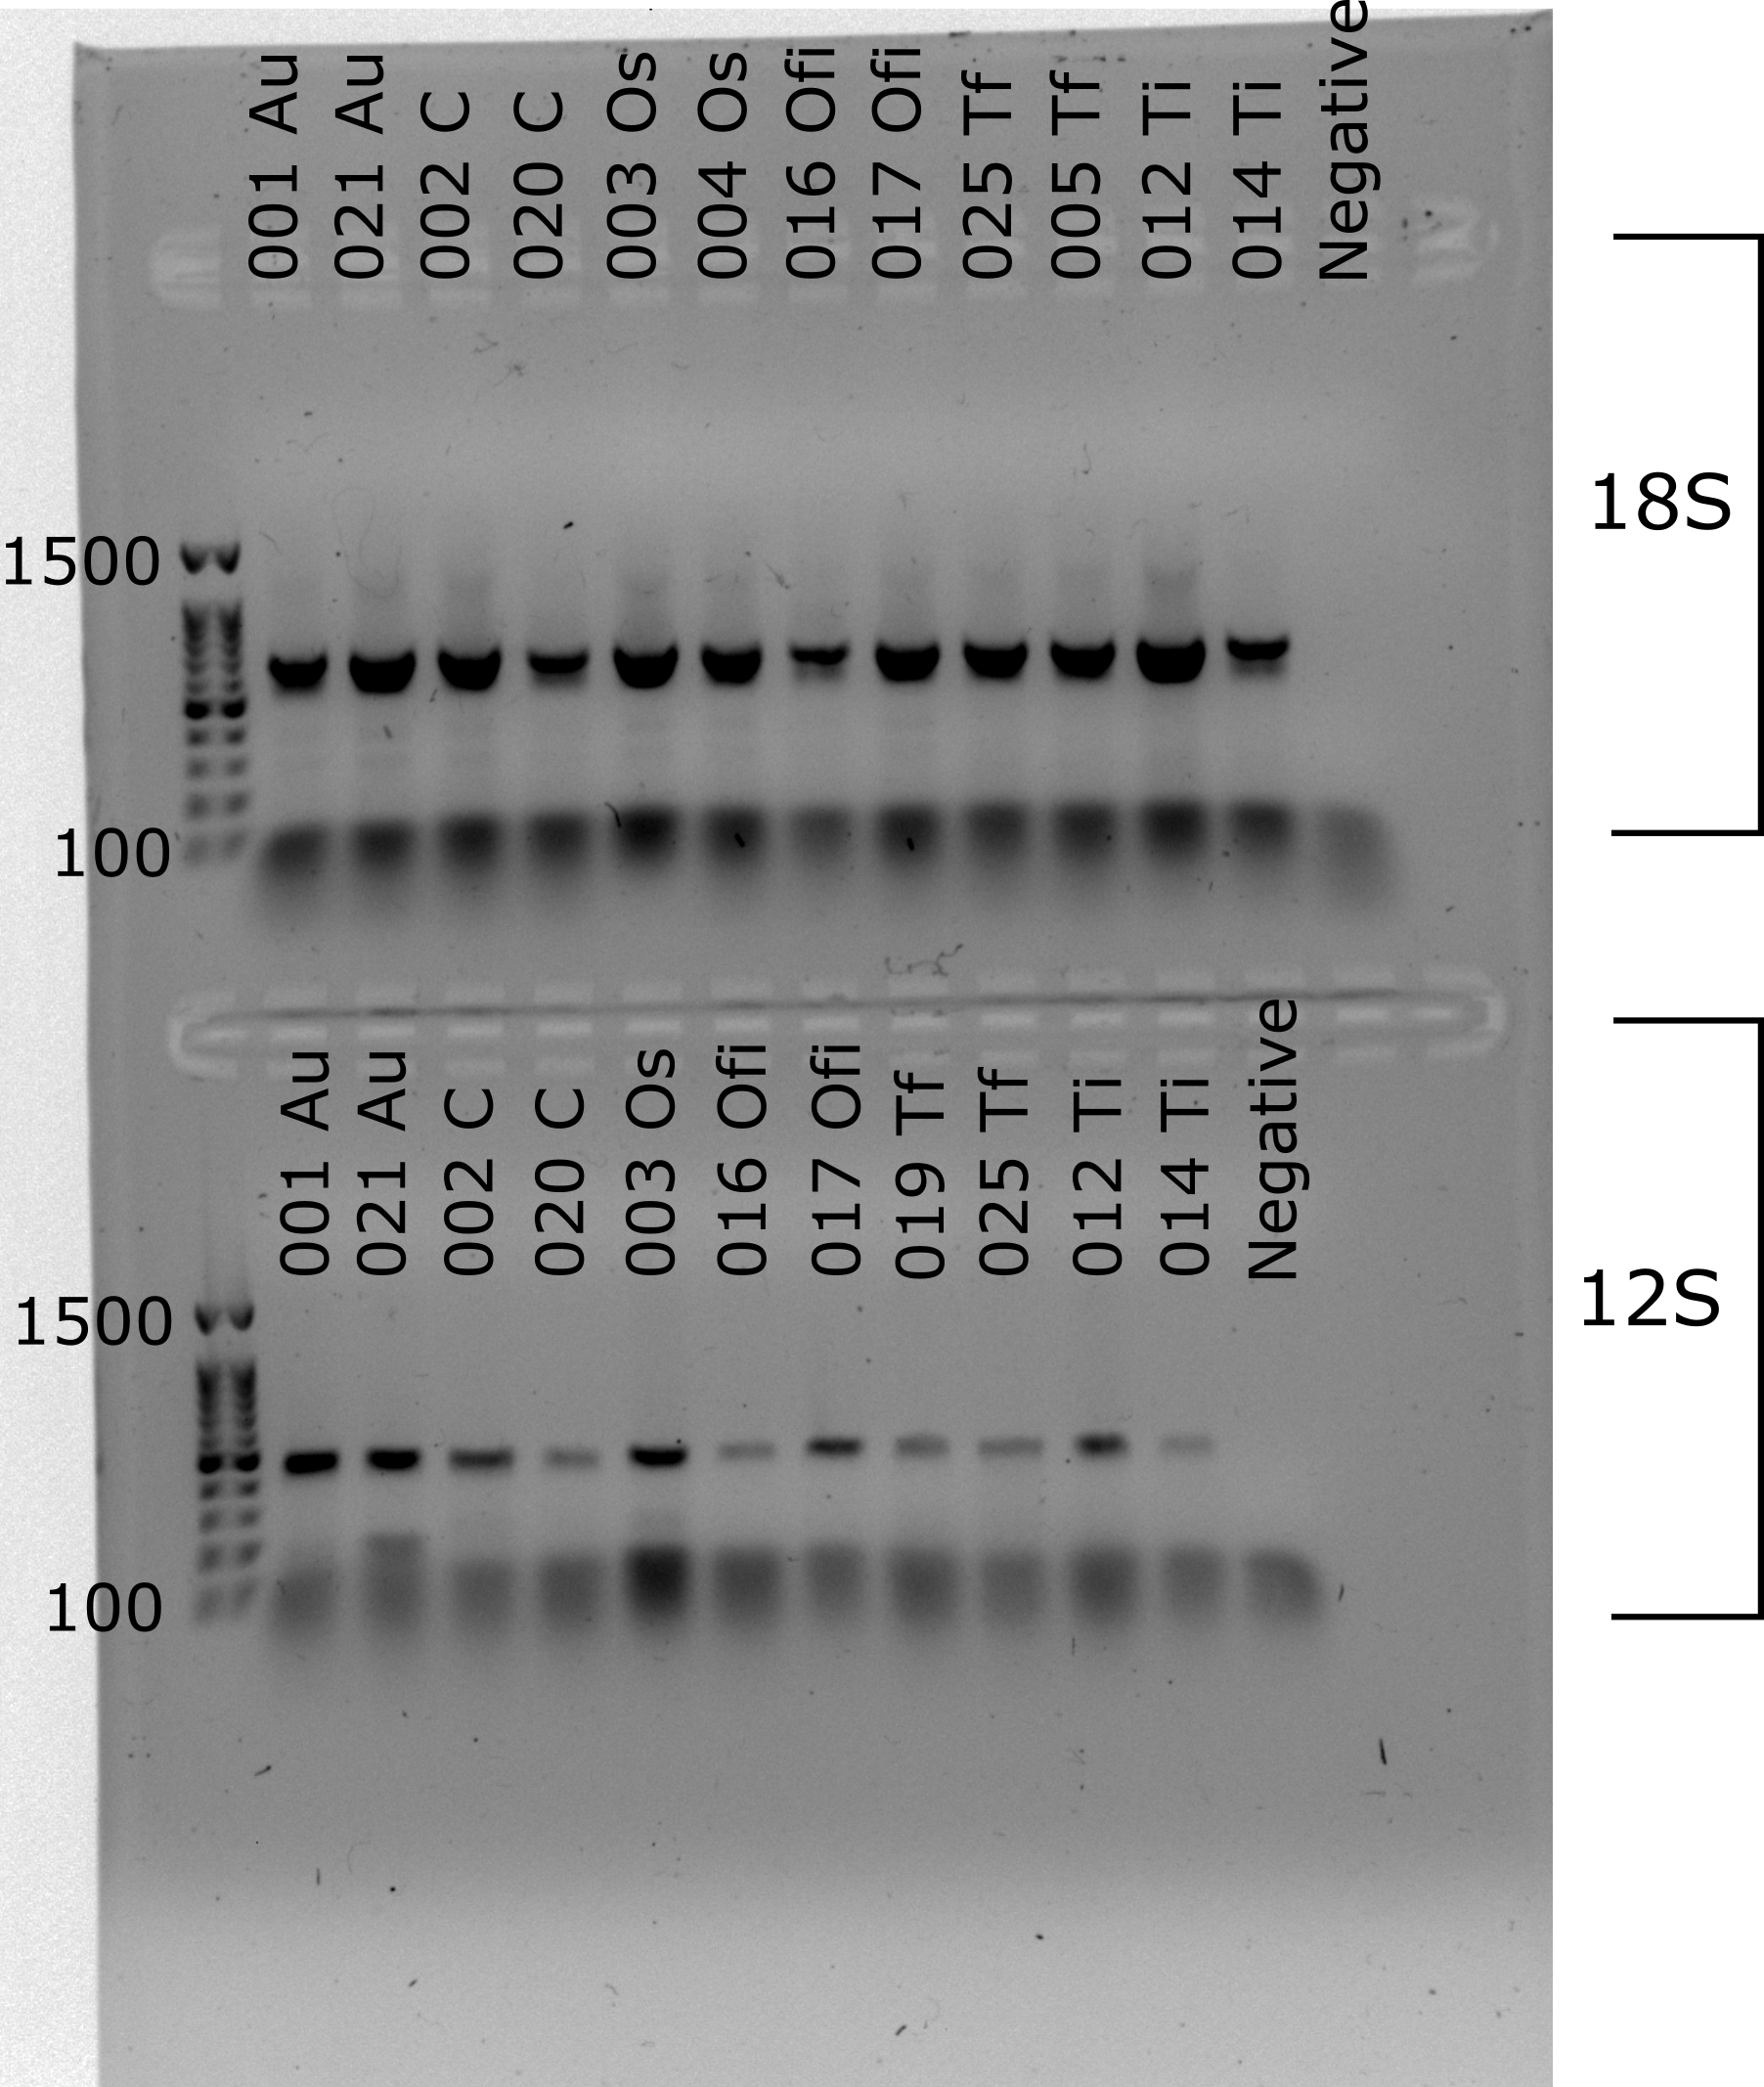
\includegraphics[scale = 1.3]{Images/12S_and_18S_gel}
%	\caption{Successful amplification of 12S and 18S genes}
%	\label{fig:gel1}
%\end{figure}

\subsection{Gel electrophoresis}
Gels were prepared using 100 mL TBE buffer (1X), 1 g Seakem\textsuperscript{TM} agarose (1\%) and 10 $\mu$L ethidium bromide. A 2 $\mu$L aliquot of loading buffer (PCRBIO Loading Buffer A) was added to 5 $\mu$L of each DNA sample. A 2 $\mu$L DNA ladder (PCRBIO Ladder IV, PCRBIOSYSTEMS) served as a standard. Gels were run at 90 V for 40 minutes using a Bio-Rad Powerpac\textsuperscript{TM}. Bands were visualized on a Bio-Rad Geldoc\textsuperscript{TM} molecular imager system and photographed using Image Lab\textsuperscript{TM} software. Amplified PCR products were sent to Macrogen Inc. in the Netherlands for purification, and for sequencing in the forward direction in all cases. 
% Relevant forward primer aliquots, diluted down to a concentration of 5 $\mu$M, were provided with the samples. 
% such that for n samples, n+5$\mu$L primer (at the original 10$\mu$M) was added to n+5 $\mu$L ddH\textsubscript{2}O.

\subsection{Sequence alignment}
Chromatograms were opened in Chromas v2.6.4 (Technelysium Pty Ltd.), where the beginning and ends of sequences were trimmed accordingly ($\pm$ 50 - 70 bp). These were subsequently opened in BioEdit v7.0.5 \citep{Hall1999BioEdit:95/98/NT}, and their base calls verified against their corresponding chromatograms. Sequences were aligned online using MAFFT v7 \citep{Katoh2017MAFFTVisualization}. The MAFFT alignment method was chosen based on the review by \citet{Morrison2006L.Purposes}, which found this method to be the most accurate and consistent compared to the ProAlign, ClustalW, T-coffee, Muscle, and Clustal methods. \\
As an additional analysis, the 12S rRNA sequences were aligned according to their predicted secondary structures using R-Coffee \citep{moretti2008, wilm2008} on the \href{http://tcoffee.crg.cat/apps/tcoffee/index.html}{T-Coffee server} \citep{notredame2000t, di2011t}. Sequences that did not show high consistencies were removed from the alignment. \\
Final sequences were submitted to Genbank via the online submission portal available at \url{https://submit.ncbi.nlm.nih.gov/}. See Section \ref{appendix:genbank_submission} for more details regarding the Genbank submission process.

\subsection{Construction of phylogenetic trees}
jModelTest v2.1.10 \citep{Guindon2003ALikelihood., Darriba2012JModelTestComputing} was used to select appropriate evolutionary models for the 12S, 18S, and COI gene regions, followed by the use of Bayesian Inference and Maximum Likelihood methods to create phylogenies for each. A concatenated phylogeny was made for the 12S and 18S regions. The COI region was not included in this concatenation, because it contained only 49\% of the sequences represented by the 12S and 18S datasets. A test concatenated phylogeny with all three genes did not show well-resolved clades within \textit{D. tomentosus}. \\
Maximum Likelihood \citep{Felsenstein1981EvolutionaryApproach} phylogenies were created using GARLI v2.01 \citep{zwickl2006genetic}, and Bayesian phylogenies were created using MrBayes v3.2.6 \citep{Huelsenbeck2001MRBAYES:Trees.} via the CIPRES Science Gateway portal \citep{Miller2010CreatingTrees} (\url{http://www.phylo.org/}). Trees were viewed in FigTree v1.4.3 and edited in Inkscape v0.92.3. 

\subsubsection{Bayesian Inference and Maximum Likelihood}

MrBayes was run using random starting trees, four chains (three hot and one cold) and set to 50 million generations. Trees were sampled every 1000 generations with a burnin of 1250 (see Section \ref{appendix:bayesblocks} for the MrBayes Nexus files used for each gene region). Tracer v1.7 was used to check for MCMC convergence \citep{rambaut2018posterior}. \\ 
% \begin{figure}[H]
% 	\centering
% 	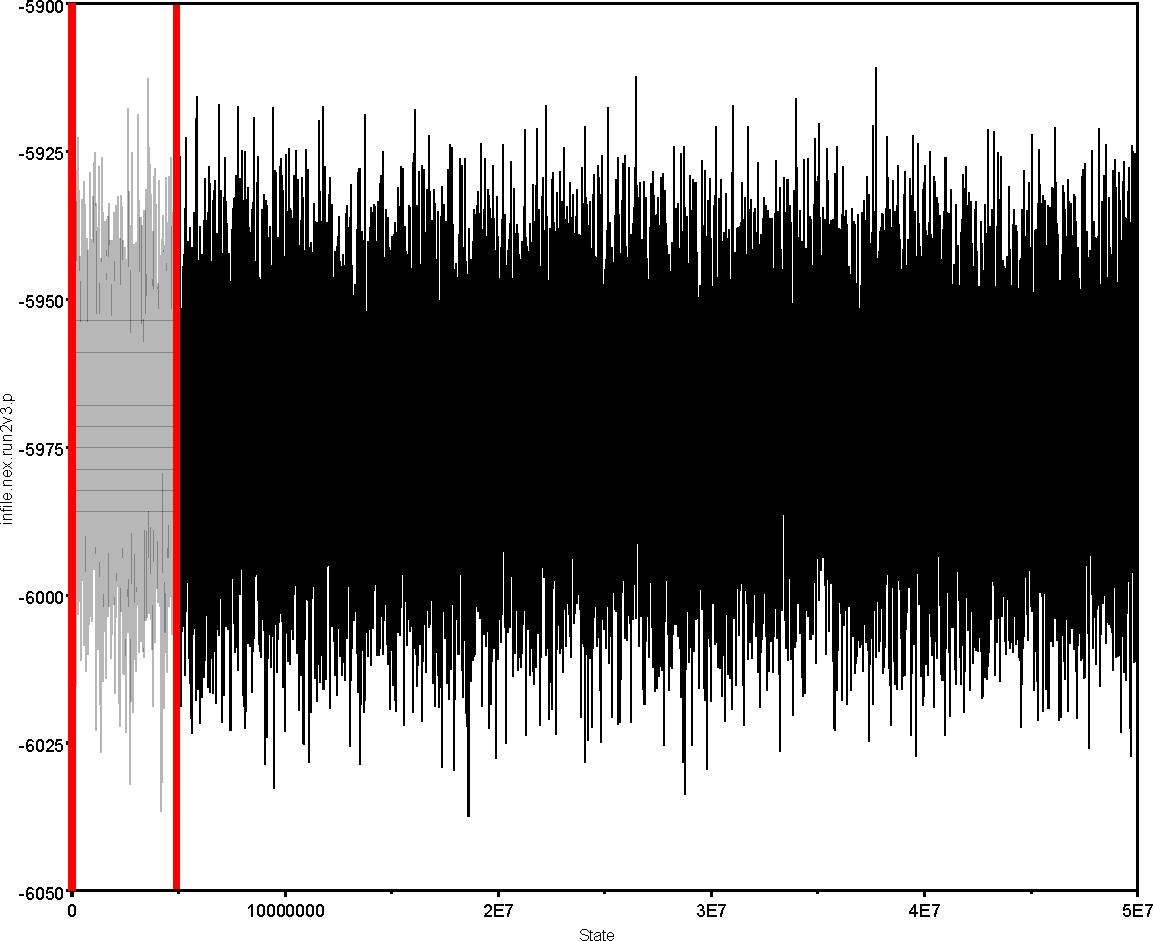
\includegraphics[scale = 0.32]{Images/tracer.pdf}
%     \newline
% 	\caption{An ideal tracer diagram indicating MCMC convergence. Burnin is the grey area between the two vertical red lines.}
% 	\label{fig:tracer}
% \end{figure}
Protein-coding COI sequences were assessed for substitution saturation at positions 1, 2, 3, and 1 \& 2 using the tests created by \citet{xia2003index} and \citet{xia2009assessing} in DAMBE v6 \citep{xia2018dambe7}. It is important to check for codon saturation, because the actual genetic distances in a dataset could be significantly underestimated due to multiple substitutions having taken place \citep{philippe2011resolving}. 
Sequences were ensured to be in the longest open-reading frame using BioEdit v7.0.5.3. 
% A significant p-value and an index of substitution saturation (ISS) less than the critical index of substitution saturation (ISSc) indicates little saturation, and that a partition model for that particular codon position is not required. 
GARLI and CONSENSE were used for the construction of Maximum Likelihood phylogenies via CIPRES. One thousand bootstrap repeats were run with two search repetitions. \\
Topologies of the individual gene trees for the 12S and 18S gene regions were compared using the online congruency index test `Icong', developed by \citet{devienne2007congruence}. To do this, a neighbour-joining tree was created for each gene region in MEGA v7 \citep{mega7} using the default settings. A significant p-value in `Icong' supports congruency, and thus the concatenation of the two relevant genetic datasets. 

\subsubsection{Haplotype networks in POPART}
POPART v1.7 \citep{leigh2015popart} was used to create 12S and COI haplotype networks for \textit{D. opuntiae} and \textit{D. confusus} using the TCS network method \citep{clement2000tcs}. \textit{Dactylopius tomentosus} haplotypes were not presented here because the 12S and COI phylogenies sufficiently represented the different lineages. It was, however, used to report the number of nucleotide differences between lineages of interest in this species. 
The 18S gene did not provide enough intraspecific variation, and was therefore not included. See Section \ref{appendix:popart} for the relevant file input formatting for POPART.
% The program was also used to calculate nucleotide diversity ($\pi$), the total number of segregating sites and Tajima's D statistic. 

\subsection{Distance-based testing of barcodes}
 The accuracy of barcode sequences were tested using the SPIDER package \citep{Brown2012Spider:Barcoding} in R v3.6.1 \citep{RCoreTeam2013R:Computing} at both the species and lineage level. This entailed the use of the Nearest Neighbour (NN), Threshold Identification (TID), and Best Close Match (BCM) methods. The threshold percentage used in TID was optimised to minimise cumulative error (false negatives + false positives). This was done by testing a range of threshold values from 0.0001\% to 2.5\% in increments of 0.005\% using the threshold optimisation function in the package. Pairwise distances were calculated using the K80 substitution model, using the dna.dist function in the R `Ape' package \citep{Paradis2004APE:Language}. The genetic barcoding gap was calculated and plotted using the SPIDER package by calculating the largest intraspecific and the smallest interspecific genetic distance for each sequence \citep{Meier2006DNASuccess}. See Section \ref{appendix:RCODE,SPIDER} for the R code used to implement these tests.
 
\subsubsection{Nearest Neighbour (NN)}
The NN algorithm was used to compare the genetic distance of each sequence of interest (treating it as a query sequence) to every other sequence in the relevant dataset. This method found the sequence that was most similar to it, and then checked whether this most similar sequence was conspecific or not. This was based upon the predefined species names, which returned a `true' or `false' result. In this way, the accuracy of each species' identification was tested and converted into a percentage of positive and negative outcomes. 

\subsubsection{Threshold ID (TID)}
The TID algorithm was used to find all the sequences that were within a genetic distance threshold of the query sequence, and returned `correct', `incorrect', or `no id' based on whether those matches were conspecific to the query sequence or not. The distance threshold was 1\% by default, but was set to an optimal value that minimised false positive and false negative results. 

\subsubsection{Best Close Match (BCM)}
The BCM algorithm was used in addition to the NN and TID, but instead of narrowing down all the matches within the genetic distance threshold, it only compared to the single nearest neighbour. It also returned `correct', `incorrect', or `no id' as output. The ambiguous output `no id' was returned when more than one sequence matched the query, where these matches included both conspecific and allospecific individuals. 
\subsubsection{Scoring of the barcode algorithms}
As per the methods of \citet{Birch2017TestingAustralia} and the R SPIDER documentation \citep{Brown2012Spider:Barcoding}, species and lineage identifications were considered: 
\vspace{0.4cm}

\begin{enumerate}
    \item ``True" in NN when the closest individual to the query was conspecific,  and ``correct" in BCM and TID analyses when all individuals with the closest distance to the query were conspecific and fell within the threshold applied.
    \item ``Ambiguous" in BCM analyses when different allospecific individuals shared the closest distance to the query and were within the threshold value or in TID analyses when different allospecific individuals were within the threshold value.
    \item ``No identification" in BCM and TID analyses when individuals were genetically more distant to the query than the threshold value.
    \item ``False" in NN when the closest individual to the query was allospecific, and ``incorrect" in BCM analyses when allospecific individuals shared the closest distance to the query and were within the threshold value or in TID analyses when all individuals within the threshold value were allospecific.
\end{enumerate}
\vspace{0.4cm}

\section{Inter-simple Sequence Repeats (ISSRs)}

\subsection{PCR protocol, data capturing and data processing}

Universal ISSR primers 809 (5'- AGA GAG AGA GAG AGA GC - 3') and 826 (5'- ACA CAC ACA CAC ACA CC -3') from Primer set \# 9 of the University of British Columbia Nucleic Acid Protein Service Unit  were used \citep{Abbot2001}. These were labelled with 5'6-FAM\textsuperscript{TM} fluorescent dye. PCRs were run in 20 $\mu$L reactions, consisting of 10 $\mu$L iTaq\textsuperscript{TM}, 1.5 $\mu$M primer and 1 $\mu$L DNA template (50 - 150 ng/$\mu$L). The PCR protocol was adapted from that of \citet{saha2011genetic} and \citet{silva2013genetic}, and carried out as per Table \ref{tab:PCRprotocol_ISSR}. 
A replication of each sample was conducted in a different PCR machine in order to validate the occurrence of bands/peaks \citep{Taylor2011GeneticMiridae, Sutton2017GeneticAgents}. As a preliminary validation step, 5 $\mu$L PCR product was run on a 1.5\% agarose gel at 6 V/cm for 3 hours (Fig. \ref{fig:issrGel}).
Samples were subsequently sent to the Central Analytical Facilities (CAF) division in Stellenbosch, South Africa, where DNA fragment analysis was performed using capillary electrophoresis (Applied Biosystems Inc., 3130 genetic analyser, GS500LIZ size standard).

\vspace{0.5cm}

\begin{table}[H]
\renewcommand{\arraystretch}{0.5}
	\centering
	\caption{PCR protocol for the ISSR 809 and ISSR 826 primers for \textit{Dactylopius} spp.}
	\label{tab:PCRprotocol_ISSR}
	\begin{tabular}{@{}clcc@{}}
		\toprule
		\textbf{Cycles} & \multicolumn{1}{c}{\textbf{Step}} & \textbf{Temperature (\textsuperscript{o}C)} & \textbf{Time} \\ \midrule
		1 & Initial denaturation & 95 & 7 min \\ \hline 
		\multirow{3}{*}{38} & Denaturation & 95 & 45 sec \\ 
		& Annealing & 44 (ISSR 809); 48 (ISSR 826) & 45 sec \\
		& Extension & 72 & 2 min \\ \hline 
		1 & Final extension & 72 & 7 min \\ \hline
		1 & Hold & 12 & $\infty$ \\ \bottomrule
	\end{tabular}
\end{table}

\subsection{ISSR data processing and analysis}

% \textbf{Summary: \newline \newline 
% \fbox{\parbox{\textwidth}{%
% Electropherograms uploaded to GeneMarker\textsuperscript{\textregistered} $\rightarrow$ Filtering of peaks above a 50RFU threshold $\rightarrow$ Creation of a peak summary table $\rightarrow$ Exportation to RawGeno for further filtering (100 RFU threshold) and binning (0.5-1bp) $\rightarrow$ Exportation of a binary matrix $\rightarrow$ Consolidation of ISSR replicates $\rightarrow$ Conversion of the binary matrix to a distance matrix using Jaccard's transformation $\rightarrow$ Creation of a hierarchical clustering dendrogram (UPGMA method) and nMDS plot in R and a NeighborNet tree in SplitsTree $\rightarrow$ Importation of the binary matrix into STRUCTURE to assess distinct genotypic clusters $\rightarrow$ STRUCTURE SELECTOR to find the optimal K-value (the best estimate of the number of genotypic clusters) $\rightarrow$ CLUMPAK (CLUster Markov Packager Across K) to visualise results as histograms.}
% }}
% \newline 
\subsubsection{Electropherograms to binary data}
Electropherograms were analysed in Genemarker\textsuperscript{\textregistered} v2.7.4 (SoftGenetics\textsuperscript{\textregistered}) (Fig. \ref{fig:overlay_electro}). 
See Section \ref{appendix:genemarker_settings} for more details regarding the settings applied.
Binary data from GeneMarker\textsuperscript{\textregistered} were opened in RawGeno v2.0 \citep{arrigo2012automated}. The following parameters were found to be the most efficient, while remaining conservative: 
\vspace{0.4cm}
\begin{enumerate}
    \item Maximum and minimum bin width of 1 and 0.5 base pairs (bp), respectively.
    \item Scoring from 100 to 500 bp.
    \item Low relative fluorescent units (RFU) of 100, as recommended by \citet{DNAFragAnalysis} for data produced by 3130 Series instruments.
\end{enumerate}
\vspace{0.4cm}

\noindent The resulting binary matrix was organised in Microsoft Excel\textsuperscript{\textregistered} and converted to a pairwise distance matrix in R using Jaccard's distance transformation. This transformation was applied because it does not consider the shared absence of bands as being biologically meaningful (Fig. \ref{fig:jaccard}) \citep{jacc}. See Section \ref{appendix:RCODE,Jaccard} for the relevant R code used to calculate distance matrices applying Jaccard's transformation. The Jaccard's distance (dJ\textsubscript{i}), and similarity (J\textsubscript{i}) index calculations are shown below, where f\textsubscript{11} represents the total number of times that a band occurred at the same place in both samples, f\textsubscript{00} represents the shared absence of bands, and f\textsubscript{10} and f\textsubscript{01} represents the number of times that a band was present in only one of the two sample replicates. Jaccard's distance is equal to 1 - Jaccard's similarity (J\textsubscript{i}). 
\vspace{0.4cm}

\[dJ\textsubscript{i} = \frac{f\textsubscript{01} + f\textsubscript{10}}{f\textsubscript{01} + f\textsubscript{10} + f\textsubscript{11}} = 1 - J\textsubscript{i} \] 

\[J\textsubscript{i} = \frac{f\textsubscript{11}}{f\textsubscript{01} + f\textsubscript{10} + f\textsubscript{11}} \] 

\subsubsection{Grouping methods}
The transformed distance matrix was subsequently used to create a hierarchical clustering dendrogram using the unweighted pair group method with arithmetic mean (UPGMA, 1000 bootstraps) using the `pvclust' R package \citep{suzuki2006pvclust}. See Section \ref{appendix:RCODE,upgma} for the R code used to construct this dendrogram. Further ISSR clustering and statistical analyses were applied to the \textit{Dactylopius opuntiae} `ficus' and `stricta' lineages in particular, as the traditional DNA barcoding regions could not differentiate between them.
Kruskal's non-metric multidimensional scaling (nMDS) method was applied using the isoMDS function in the MASS package in R \citep{MASS_R}. See Section \ref{appendix:RCODE, nmds} for the relevant R code used to create the nMDS plot. Dimensions K = 2 and K = 3 were tested, and the one yielding the lowest stress value was selected. The use of an nMDS ordination method was confirmed using stress and Shepard plots. 
% A stress plot shows how the number of dimensions of an MDS ordination affects the stress value, which is a measure of goodness of fit. The lower the stress value, the better the fit \citep{clarke1993}. A Shepard plot illustrates the relationship between the distance data before and after the ordination method has been applied. Ideally, the resulting regression should yield a high R\textsuperscript{2} value and show a significant correlation. \newline
An ANOSIM (ANalysis Of SIMilarity) was applied to lineages and populations using the `vegan' package in R \citep{vegan_R}, using 999 permutations \citep{clarke1993}. Pairwise p and R-values were obtained from PAST v3 \citep{Hammer2001PAST:Analysis}. 
% where a large positive R-value indicates a high level of dissimilarity, and a smaller value indicates increasing similarity. 
In addition to the ANOSIM, a Permutational Multivariate Analysis Of Variance (PERMANOVA) using distance matrices was used, applying the adonis function in the `vegan' package, with 999 permutations. This test is less sensitive to within-group heterogeneity \citep{anderson2014permutational}. Post-hoc pairwise comparisons were obtained via the pairwise.perm.manova function in the `RVAideMemoire' package \citep{herve2015rvaidememoire}. See Section \ref{appendix:RCODE,anosim,permanova} for the R code used to output the ANOSIM and PERMANOVA test results. \\
Data were also imported to SplitsTree4 v4.15.1 \citep{huson2006splitstree}, and used to create NeighborNet trees based on distance matrices that were transformed using Jaccard's distance index. NeighborNet trees were chosen because \citet{huson2006splitstree} suggest that this method produces highly resolved networks. See Section \ref{appendix:splitstree_input} for the SplitsTree file input format. 

\subsubsection{STRUCTURE}
STRUCTURE v2.3.4 \citep{Pritchard2000InferenceData, evanno2005detecting} was used to analyse the genetic clustering of \textit{D. opuntiae} samples. 
% This particular species was used because the traditional DNA markers did not show a separation between the `ficus' and `stricta' lineages. 
The program uses Bayesian analysis and the Markov Chain Monte Carlo (MCMC) estimation method to assign individuals to genotypic cluster groups (\textit{K}) \citep{Pritchard2000InferenceData}. 
% The method assumes that the input loci are in Hardy-Weinberg and linkage equilibrium, and does not consider any particular underlying mutation processes \citep{structureManual2009}.
STRUCTURE was run twice; once where the population origins for samples were given as priors (`PopData'), and once where they were not. 
% This was done through selecting the `use sampling locations as prior' option in the parameter settings.
See Section \ref{appendix:structure_settings} for details regarding the specific settings used. 
The results obtained from STRUCTURE were uploaded to STRUCTURE SELECTOR \citep{li2018structureselector}, which finds the best estimate of the number of genetic cluster groups (\textit{K}-value) present. The Peuchmaille method was preferred for this analysis, as it was found to outperform previous methods for datasets containing both even and uneven sample sizes \citep{puechmaille2016program}. \citet{puechmaille2016program} developed four statistical tests to estimate the optimal \textit{K}-value for a dataset, namely `MedMeaK', `MaxMeaK', `MedMedK', and `MaxMedK'. 
% The algorithm calculates mean and median membership coefficient values for each sample, compares it to a threshold (where a higher threshold implements a higher stringency), and assigns it accordingly to a cluster group. The mean and median number of cluster groups are subsequently estimated. 
The present analysis set the threshold to range between 0.5 and 0.8, as per the recommendations of \citet{puechmaille2016program}. The \textit{K}-estimation according to the conventional Evanno method \citep{evanno2005detecting} was also reported. CLUMPAK software \citep{Kopelman2015} was used to visualise results. 

% \subsubsection{POPGENE}
% POPGENE \citep{yeh1997population} was used to calculate the total number of alleles (na), effective number of alleles (ne), Nei's genetic diversity (h), Shannon's information index (I), polymorphic loci, total genetic diversity (Ht), intra population genetic diversity (Hs) and the coefficient of gene differentiation (Gst) for \textit{D. opuntiae} samples. This was done for each individual primer, as well as for their concatenation. See Section \ref{appendix:popgene_input} for details regarding the file input format.

\subsubsection{ISSR error rates}

Two genoytyping error rates were calculated, namely the `Euclidean' (EE) and `Jaccard' (JE) errors, as suggested by \citet{bonin2004track}, \citet{pompanon2005genotyping}, and \citet{holland2008optimizing}. \newline 
\[EE = \frac{f\textsubscript{10} + f\textsubscript{01}}{f\textsubscript{10} + f\textsubscript{01} + f\textsubscript{11} + f\textsubscript{00}} \] 
 
\[JE = \frac{f\textsubscript{10} + f\textsubscript{01}}{f\textsubscript{10} + f\textsubscript{01} + f\textsubscript{11}} \]
 
\noindent Due to the JE not taking the shared absence of bands into account, it will be inflated if the data contain numerous band-absent loci.

\section{Graphical User Interface (GUI) Applications}

\subsection{R Shiny Applications}
R Shiny applications \citep{shiny} are hosted on Amazon's Web Services online platform, and the front end can be accessed by any user via a unique url link. Running the program only requires an Internet connection, and does not rely on any pre-installed R software or related packages. Each Shiny application comprises of a user interface object (ui.R) and a server function (server.R), which are uploaded to a profile on \url{https://www.shinyapps.io/}. Three such applications were created and are described below. A help file accompanies each application. 

\subsection{Barcode Testing}
An application that allows a user to apply barcode testing algorithms to a set of aligned FASTA sequences (Fig. \ref{fig:barcodeTesterGUI}) is available at \url{https://clarkevansteenderen.shinyapps.io/BarcodeTester/}. The barcode tests were taken from the SPIDER package developed by \citet{Brown2012Spider:Barcoding}. The user can also view and download a heat map representation of a distance matrix, plots for base frequencies and GC content (using the `Ape' package \citep{Paradis2004APE:Language}), and a UPGMA clustering tree in the case of binary data.  

\subsection{Binary data processing: `BINMAT'}
A second GUI application (Fig. \ref{fig:binmatGUI}) was created in order to rapidly consolidate replicate pairs in a binary matrix containing fragment analysis data from a dominant genetic marker such as an ISSR or AFLP analysis (i.e. it requires already-scored data from a program such as GeneMarker\textsuperscript{\textregistered}). The algorithm combines replicates such that if a band was only present in one replicate (``0'' and a ``1''), it is treated as ambiguous (scored as a ``?''). The dual presence or absence of a band remains a ``1'' or ``0'', respectively. The application also calculates the average Euclidean and Jaccard error rates with standard deviations, and outputs the average, minimum, and maximum number of peaks and their standard deviations. An option is provided for constructing a UPGMA clustering tree to preview the clustering pattern of the data.
An additional feature allows the user to upload their consolidated matrix to create an interactive nMDS plot that can be downloaded as a .svg file. Options are available to view scree and Shepard plots for the data, download the distance matrix, and remove samples with total peak numbers below a specified threshold value. These filtered datasets can be downloaded and re-uploaded to create new nMDS plots. 
The BINMAT application is accessible at \url{ https://clarkevansteenderen.shinyapps.io/BINMAT/}.

\subsection{Identification of query sequences: `Dacty-ID'}

The third GUI application allows the user to paste a query nucleotide sequence into a search box, which is then aligned with sequences in a pre-selected database (Fig. \ref{fig:identifier_GUI}). The databases are the sequences for the 12S, 18S, and COI gene regions (COI-A and COI-B) obtained in this project. Alternatively, the user can upload their own set of sequences to serve as a database. A phylogenetic tree is subsequently created, where the position of the query sequence is highlighted in red relative to the database. The Dacty-ID application is available at
\url{ https://clarkevansteenderen.shinyapps.io/Dactylopius_ID_version_1/}. 
